\documentclass[8pt]{beamer}
\usetheme{default} % Very simple theme
\usecolortheme{dove} % Minimalist grayscale colors
\setbeamertemplate{navigation symbols}{} % Remove navigation bar

% Define brand-like colors
\definecolor{myblue}{RGB}{0, 102, 204}    % Blue for standard blocks
\definecolor{mygreen}{RGB}{0, 153, 0}     % Green for example blocks
\definecolor{myred}{RGB}{204, 0, 0}       % Red for alert blocks
\definecolor{myorange}{RGB}{255, 128, 0} % For \emph

% Accent color for titles, bullets, etc.
\setbeamercolor{structure}{fg=myblue}

% Block colors
\setbeamercolor{block title}{bg=myblue, fg=white}
\setbeamercolor{block body}{bg=blue!5, fg=black}

\setbeamercolor{exampleblock title}{bg=mygreen, fg=white}
\setbeamercolor{exampleblock body}{bg=green!5, fg=black}

\setbeamercolor{alertblock title}{bg=myred, fg=white}
\setbeamercolor{alertblock body}{bg=red!5, fg=black}
\setbeamercolor{alerted text}{fg=myred}

% Optional: color for \example text
\setbeamercolor{example text}{fg=mygreen}

% Custom emph (orange text instead of italic)
\let\oldemph\emph
\renewcommand{\emph}[1]{\textcolor{myorange}{#1}}


\usepackage{graphicx} % Package for images
\usepackage{amsmath} % Package for images
\graphicspath{{figs/}} % Path to your figures directory
\usepackage{array}  % For better column spacing
\usepackage{caption} % Required for \captionof

% Title Information
\title{STOCHASTIC METHODS IN WATER RESOURCES}
\vspace{25pt}
\subtitle{Unit 1: Introduction to probability and statistics \\ Lecture 5: Model estimation and testing}
\author{Luis Alejandro Morales, Ph.D.}
\institute{Universidad Nacional de Colombia \\ Department of Civil and Agriculture Engineering} %// }
%\date{\today}

\begin{document}

% Title Slide
\begin{frame}
    \titlepage
\end{frame}

%-------
% From Kotte
\section{Generalities}
\begin{frame}{Generalities}
    \begin{itemize}
        \item Statistical inference deals with  statistical estimations based on a \emph{sample} from the \emph{population}.
        \item Some definitions:
            \begin{itemize}
                \item \alert{Population}: consist of all possible observations of a process (e.g. air temperature at certain location). Some of the observations in the in the population may not have any physical sense, perhabs, due to sensor errors. 
                \item \alert{Sample}: is a subset of the population (e.g. instantaneous daily streamflow for a certain period in a station). A \emph{random sample} is thus a sample that is representative of the population.
                \item \alert{Random variables}: is a \emph{real-valued function} defined on a \emph{sample space}. Wheather a random variable is \emph{discrete} or \emph{continuous} depends on how the sample space is defined. 
                \item \alert{Statistic}: is a function of the observations that is quantifiable and does not contain any unknown parameter. Note that a \emph{statistic} is also a random variable that provides an \emph{estimation}.
                \item \alert{Estimator}: is the method or rule of estimation. For instance, the \emph{sample mean} $\bar{X}$ is a point estimator of the \emph{population mean} $\mu$. 
                \item \alert{Estimate}: is the value yielded by the estimator. 
                 \end{itemize}
             \item Suppose that the population of variable $X$ follows a \emph{Normal distribution} and the distribution parameters $\theta$ are unknown. Thus, a random sample of $X$ of size $n$.
             \item Parameters $\theta$ can be described by a number or a range; this last include an uncertainty. 
    \end{itemize}
\end{frame}

%-------
% From Kotte
\section{Properties of estimators}
\begin{frame}{Properties of estimators}
    
    \begin{block}{Unbiasedness}
        Given a sample of observations of a random variable $X$, $X_1, X_2, \cdots, X_n$, the objective is to estimate the value of the parameter $\theta$, which is also a random variable. The idea is to seek for a \emph{estimator} of  $\theta$ that get as closest as possible to the \emph{true value}. This estimator will produce statistics that are distributed following a certain \emph{pdf}. Following this, a \alert{point estimator $\hat{\theta}$}  is an \alert{unbiased estimator} of the population parameter $\theta$ if $E[\hat{\theta}] = \theta$. If the estimator is biased, the $\text{bias} = E[\hat{\theta}] - \theta$.
    \end{block}
    
    \begin{exampleblock}{Mean of the sample mean}
        Let us show that the sample mean $\bar{X}$ is an unbiased estimator of $\mu$. If $\bar{X} = \frac{1}{n} \left( X_1 + X_2 + \cdots + X_n \right) $, then $E[\bar{X}] = \frac{1}{n} nE[X_i] = \frac{1}{n} (n \mu) = \mu$. 
    \end{exampleblock}
    Note that many estimator are biased and methods such as \emph{jackknife} and \emph{bootstrap} are used to reduce the bias. Ideal estimator must also have the following properties. 
    \begin{block}{Consistency}
        An estimator $\hat{\theta}_n$, based on a sample size $n$, is a \alert{consistent} estimator of $\theta$ if for any positive number $\varepsilon$ $\lim_{n\rightarrow \infty} Pr[ | \hat{\theta}_n - \theta | \leq \varepsilon ] = 1$
    \end{block}

    \begin{block}{Minimum variance}
        A part for looking for an unbiased estimator, it is also desirable to seek for an \alert{minimum variance estimator}. The \emph{minimum variance unbiased estimator} is the estimator with the smallest variance out of all unbiased estimator
    \end{block}


\end{frame}
    

\begin{frame}{Properties of estimators}
\begin{block}{Efficiency}

    \vspace{-5pt}
    \alert{Efficiency} is the relative measure of the variance of the sampling distribution, with the efficiency increasing as the variance decrease. In terms of the \emph{mean square error (mse)} an estimator with the minimum $mse$ among all possible unbiased estimators is called and \alert{efficient estimator}. If $A$ is an estimator of $\theta$, the $mse$ is:
    \begin{align*}
        E\left[(A-\theta)^2\right] &= E\left[ \left( \left(A - E[A] \right) - \left( \theta - E[A] \right) \right)^2 \right]  \\
                                                                                                                                  &= E[ (A - E[A])^2 ] + (\theta - E[A])^2 \\
                                                                                                                                  &= Var[A] - bias^2
    \end{align*}
    The $mse$ of an estimator can be used as a relative measure of efficiency when comparing two or more estimator. 
    \end{block}

    \vspace{-7pt}
\begin{block}{Sufficiency}
    So far, properties such as unbiasedness, consistency and the minimum $mse$ are key to select the most suitable estimators. Thus, a \alert{sufficient estimator} provides as much information as possible about a sample of observations of a random variable $X$. Let a sample $X_1, X_2, \cdots, X_n$ be drawn randomly from population having probability distribution with unknown parameters $\theta$. Thus, the statistic $T = f(X_1, X_2, \cdots, X_n)$ is said to be sufficient to estimate $\theta$ if the distribution of $X_1, X_2, \cdots, X_n$ conditional to the statistics $T$ is independent of $\theta$.    
    \end{block}
    \vspace{-9pt}
    \begin{exampleblock}{Median and mean}
        The \emph{median}, taken as a measure of mean density or central tendency, does not contain all the information in a sample. The median is the middle value of the sample; if any other value is changed the mean changes but the median is unaltered.
    \end{exampleblock}

\end{frame}

%-------
% From Kotte
\section{Estimation of confidence intervals}
\begin{frame}{Estimation of confidence intervals}
    The uncertainty of point estimates can be quantified by the relative variances or mean square errors of the estimators. Because of this uncertainty, the next step of inference is \alert{interval estimation}. Two numbers, say, $a$ and $b$, that are expected to include within their range an unknown parameter $\theta$ in a specified percentage of cases after repeated experimentation under identical conditions. That is, in place of one statistic that estimates $\theta$, we find a range specified by two statistics, which includes it at a given level of probability. The end points $a$ and $b$ of this range are known as \alert{confidence limits}, and the interval $(a, b)$ is known as the \alert{confidence interval}. We do not have the precision as for a point estimator but we have confidence (without absolute certainty) that the assertion is right.

\begin{block}{Confidence interval estimation of the mean when the standard deviation is known}
    Let $C_l$ and $C_u$ be the \emph{lower} and \emph{upper} confidence limits that include an unknown but invariable parameter $\theta$. Although there is some uncertainty associated with this statement, we will be right in a proportion, say, $1 – \alpha$, of the samples taken from the same population, on average, when we make the assertion that the given interval includes $\theta$. Thus we can say, by adopting the long-run frequency interpretation of probability,
\[
    Pr[C_l  \leq \theta \leq C_u ] = 1 - \alpha
\]
where $\theta$ is a constant, but the estimator $\hat{\theta}$  and the confident limits $C_l$ and $C_u$ are random variables. Recall that examples of $\hat{\theta}$ are $\bar{X}$ and $\bar{S}^2$. The probability $(1 – \alpha)$ is known as the \emph{confidence level} or \emph{confidence coefficient}. It often takes values such as 0.99, 0.95, and 0.90. The confidence limits $C_l$ and $C_u$ depend on the sampling distribution of $\theta$. The standard deviation of the statistic $\hat{\theta}$ called its \emph{standard error}.

    \end{block}
\end{frame}

\begin{frame}{Estimation of confidence intervals}
\begin{block}{Confidence interval estimation of the mean when the standard deviation is known}
    In some situations, we may require \emph{one-sided confidence limits}. The \emph{lower and upper one-sided confidence limits} are specified, respectively, by
    \[
        Pr[C_l \leq \theta] = 1 - \alpha \quad \text{for } 0 < \alpha < 1
    \]
    and

    \[
        Pr[\theta \leq C_u] = 1 - \alpha \quad \text{for } 0 < \alpha < 1
    \]
\end{block}

\begin{minipage}[t]{0.54\textwidth}
   \vspace{0pt} % prevent extra spacing at top
    Let $\bar{X}$ be the mean of a random sample of size $n$ drawn from a population with known standard deviation $\sigma$. The $100(1 – \alpha)$ percent central two-sided confidence interval for the population mean $\mu$ is $\left( \bar{X} - z_{\alpha/2} \frac{\sigma}{\sqrt{n}}, \bar{X} + z_{\alpha/2} \frac{\sigma}{\sqrt{n}} \right)$, where $z_{\alpha/2}$ is a standard normal variate that is exceeded with probability $\alpha/2$, $Z = \frac{\bar{X}- \mu}{\sigma/\sqrt{n}} \quad N \sim (0,1)$. The one-sided upper and lower $100(1 – \alpha)$ percent confidence limits for the population mean $\mu$ are, $\bar{X} + z_{\alpha} \frac{\sigma}{\sqrt{n}} $ and $\bar{X} - z_{\alpha} \frac{\sigma}{\sqrt{n}} $, respectively. 
\end{minipage}
%\hfill
\begin{minipage}[t]{0.44\textwidth}
   \vspace{0pt} % prevent extra spacing at top
    \centering
    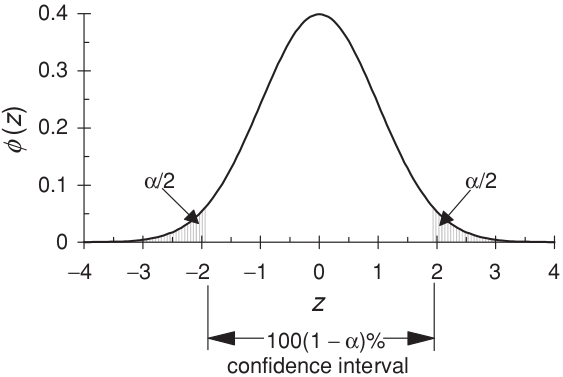
\includegraphics[width=\textwidth]{fi531.png}
\end{minipage}

\end{frame}


\begin{frame}{Estimation of confidence intervals}
    \begin{block}{Confidence interval estimation of the mean when the standard deviation is unknown}
        Quite often in practice the mean and standard deviation are both unknown. Under such conditions we must modify our approach. We assume normality of the variate $X$ as before, but the consequences of a \emph{nonnormal distribution} are minor for small to moderate departures from normality, if the sample size is large, say, $n > 30$. In this situation we apply the \emph{Student's t distribution}.The T variable represents the mean $\bar{X}$ standardized as $T = \frac{\bar{X}- \mu}{\hat{S}/\sqrt{n}} \sim t_{n-1}$. Note that $T$ has a  \emph{Student’s t distribution} with $\nu = (n-1)$ degrees of freedom. Recall that the \emph{Student's t distribution} \emph{pdf} is:
        \[
            f_T (t) = \frac{\Gamma[(\nu +1)/2]}{\sqrt{\pi \nu} \Gamma(\nu/2)} \frac{1}{\left[ (t^2 /\nu) + 1 \right]^{\frac{\nu +1}{2}}} \quad \text{for } -\infty < t < \infty
            \]

\end{block}
\begin{minipage}[t]{0.54\textwidth}
   \vspace{0pt} % prevent extra spacing at top
   Let $\bar{X}$ and $\hat{S}$ be the mean and the standard deviation, respectively,  of a random sample of size $n$ drawn from a \emph{normal distribution} with unknown standard deviation $\sigma$. The $100(1 – \alpha)$ percent central two-sided confidence interval for the population mean $\mu$ is $\left( \bar{X} - t_{n-1, \alpha/2} \frac{\hat{S} }{\sqrt{n}}, \bar{X} + t_{n-1, \alpha/2} \frac{\hat{S}}{\sqrt{n}} \right)$, where $t_{n-1, \alpha/2}$ is  \emph{Student's t variate} with $n-1$ degrees of freedom  and probability of $\alpha/2$ of execeedance. 
\end{minipage}
%\hfill
\begin{minipage}[t]{0.44\textwidth}
   \vspace{0pt} % prevent extra spacing at top
    \centering
    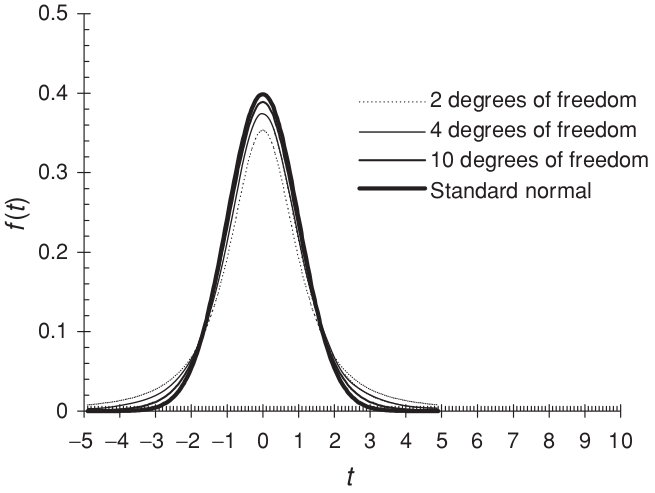
\includegraphics[width=\textwidth]{fi532.png}
\end{minipage}
\end{frame}


\begin{frame}{Estimation of confidence intervals}
    \begin{block}{Confidence interval for a proportion}
    Consider a two-sided \emph{Bernoulli} variable that occur with probability $p$ if it is success and $1-p$ if it is failure. Recall that mean and the variance of this variable are $p$ and $p(1-p)$, respectively. If an experiment involving a \emph{Bernoulli} variable is repeated $n$ times, the \emph{standard error} of the estimated proportion of a success is:
    \[ 
        \sigma_{\hat{p}} = \sqrt{\frac{p(1-p)}{n}}
    \]
    Note that for a large sample size, for instance, $n>30$, and for $np > 5$ and $n(1-p) > 5$. the sampling distribution is nearly \emph{normal}.
\end{block}

\end{frame}

\begin{frame}{Estimation of confidence intervals}
\begin{block}{Sampling distribution of differences and sums of statistics}
    Let $S_1$ and $S_2$ independent statistics from two populations, computed based on sample sizes $n_1$ and $n_2$, respectively. Let the means and the standard errors of the sampling distributions of the two statistics  be $\mu_{S_1}$, $\mu_{S_2}$ and $\sigma_{S_1}$, $\sigma_{S_2}$, respectively. The differences between the statistics (after repeated sampling) from the two populations have a sampling distribution with mean $\mu_{S_1 - S_2} = \mu_{S_1} - \mu_{S_2}$, and standard error $\sigma_{S_1 - S_2} = \sqrt{\sigma_{S_1}^2 + \sigma_{S_2}^2}$. The sampling distribution of the sum of the statistics $S_1 + S_2$ has a mean $\mu_{S_1 + S_2} = \mu_{S_1} + \mu_{S_2}$, and standard error $\sigma_{S_1 + S_2} = \sqrt{\sigma_{S_1}^2 + \sigma_{S_2}^2}$.
\end{block}
\vspace{-7pt}
    \begin{exampleblock}{Confidence limits for differences between two means of the annual rainfalls at two stations}
        At station 1, annual rainfall has been measured over $n_1 = 50$ years where $\bar{x_1} = 900$ mm and $\hat{s}_1 =80$ mm. At station 2, annual rainfall has been measured over $n_1 = 40$ years where $\bar{x_1} = 825$ mm and $\hat{s}_1 =90$ mm. Because annual rainfalls are the result of a large number of small causes, such an additive effect makes it plausible to assume that the distribution is normal. Thus, the sampling distribution of the difference between the two means is also normal. 

\begin{minipage}[t]{0.48\textwidth}
        The $(1-\alpha)$ percent confidence limits for the difference between the two means are found using:
\vspace{-14pt}
        \[
        (\bar{x}_1 - \bar{x}_2) \pm z_{\alpha/2} \sqrt{\frac{\sigma_1^2}{n_1} + \frac{\sigma_2^2}{n_2}}
    \]
    where $z_{\alpha/2}$ is the standard  normal variate  which is exceeded with probability $\alpha/2$.  
\end{minipage}
\begin{minipage}[t]{0.48\textwidth}
    Replacing $\hat{s_1}$ for $\sigma_1$ and $\hat{s_2}$ for $\sigma_2$, the 95\% confident limits are:
\vspace{-7pt}
    \[
        75 + 1.96 \sqrt{\frac{80^2}{50} + \frac{90^2}{40}} = 75 \pm 36 mm 
    \]
    limits of $(39 mm, 111 mm )$. 
\end{minipage}
    \end{exampleblock}

\end{frame}

\begin{frame}{Estimation of confidence intervals}
\begin{block}{Interval estimation for the variance: chi-squared distribution}
    Consider a set of normally and independently distributed random variates $X_i$ where $i = 1, 2, \cdots, \nu$, with means $\mu_i$ and variances $\sigma_i^2$. If we standardize the $X_i$ by subtracting the mean and dividing by the standard deviation, respectively, to a set  $Z_i$, $i =1, 2, \cdots, \nu$  with zero mean and unit variance. Consider the random variable formed by the sum of squares of the $Z$ variables, say $\chi^2 = Z_1^2 + Z_2^2 + \cdots + Z_{\nu}^2$. The \emph{mgf} of $\chi^2$ is given by:
    \[
        M_{\chi^2} (t) = E[e^{t \chi^2}] = \prod_{i=1}^\nu E[e^{t Z_i^2}]
    \]
    Regarding that:
    \[
        E[e^{t Z_i^2}] = \int_{-\infty}^{\infty} e^{tz^2} \frac{e^{-z^2 /2}}{\sqrt{2\pi}} dz = \frac{1}{\sqrt{1-2t}} \int_{-\infty}^{\infty} \frac{\sqrt{1-2t}}{\sqrt{2\pi}} e^{-(1-2t)z^2 / 2} dz 
    \]
the integral on the right-hand side is unity, being a representation of the area under a normal curve with a mean of zero and variance $1/(1-2t)$, so:
\[
    M_{\chi^2} (t) = \left[ \frac{1/2}{1/2 -t} \right]^{\nu/2}
\]

\end{block}
\end{frame}

\begin{frame}{Estimation of confidence intervals}
\begin{block}{Interval estimation for the variance: chi-squared distribution}

\begin{minipage}[t]{0.48\textwidth}
If we compare this \emph{mgf} with the one  for the gamma distribution, the \emph{cdf} of the \emph{chi-squared distribution} with $\nu$ degrees of freedom is:
\[
    F(\chi^2) = \frac{1}{2} \int_0^{\chi^2} \frac{(u/2)^{(\nu/2) -1} e^{-u/2}}{\Gamma (\nu/2)} du
\] 
\end{minipage}
\begin{minipage}[t]{0.48\textwidth}
   \vspace{0pt} % prevent extra spacing at top
    \centering
    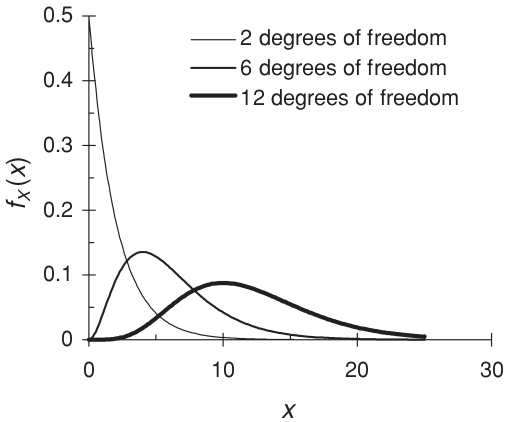
\includegraphics[width=\textwidth]{fi534.png}
\end{minipage}
Considering a random sample $X_1, X_2, \cdots, X_n$ of independent normally distributed variables with common mean $\mu$, variance $\sigma^2$ and sample mean $\hat{X}$. 
\[
    \hat{S}^2 = \frac{1}{n-1} \sum_{i=1}^n (X_i - \bar{X})^2
\]
is an unbiased estimator of the variance $\sigma^2$. Let us now consider the quantity
\[
    \sum_{i=1}^n (X_i - \mu)^2 = \sum_{i=1}^n \left[(X_i - \bar{X}) + (\bar{X} - \mu) \right]^2
\]

\end{block}
\end{frame}

\begin{frame}{Estimation of confidence intervals}
\begin{block}{Interval estimation for the variance: chi-squared distribution}
because $\sum_{i=1}^n (X_i - \bar{X})=0$, the cross-product in this equation is zero, so:
\[
    \sum_{i=1}^n (X_i - \mu)^2 = \sum_{i=1}^n (X_i - \bar{X})^2 + n(\bar{X} - \mu)^2
\]
Dividing by $\sigma^2$ and substituting $\hat{S}^2$ from the equation above for the second term:
\[
    \frac{\sum_{i=1}^n (X_i - \mu)^2 }{\sigma^2}  = \frac{(n-1)\hat{S}^2}{\sigma^2} + \frac{(\bar{X} - \mu)^2}{\sigma^2 /n}
\]
If the first term of this equation is distributed as $\chi^2_n$, and according to the \emph{Central Limit Theorem}, the last term is  distributed as $\chi^2_1$. Thus, taking account of the additive property of the gamma and chi-squared variates, we can say that $\frac{(n-1)\hat{S}^2}{\sigma^2}$ has $\chi^2_{n-1}$ distribution, that is,  with $\nu = n-1$ degrees of freedom. This important result is used in finding \emph{confidence limits} for the variance $\sigma^2$ of a \emph{normal population}. The \emph{chi-squared cdf} is given in tables for various values of the degrees of freedom $\nu$. For example, the $(1 – \alpha)$ percent two-sided confidence interval for $\sigma^2$ is found from:
\[
    Pr \left[ \chi^2_{n-1, 1- \alpha/2} \leq \frac{(n-1)\hat{S}^2}{\sigma^2} \leq  \chi^2_{n-1, \alpha/2} \right] = 1-\alpha
\]
\end{block}
\end{frame}

\begin{frame}{Estimation of confidence intervals}
\begin{block}{Interval estimation for the variance: chi-squared distribution}
\begin{minipage}[t]{0.60\textwidth}
    This probability is represented by the area between the two vertical lines of the figure which shows the \emph{pdf}. These values are from left to right the values that a $\chi^2_{n-1}$ variate exceeds with probabilities $(1-\alpha/2)$\% and $\alpha/2$\%, respectively. Taking reciprocal of the variables in the equation, the positions of the \emph{chi-squared} variables need to be  changed, and multiplying by $(n-1)\hat{S}^2$, we obtain:
\[
    Pr \left[ \frac{(n-1)\hat{S}^2}{\chi^2_{n-1, \alpha/2}} \leq \sigma^2 \leq \frac{(n-1)\hat{S}^2}{\chi^2_{n-1, 1- \alpha/2}}  \right] = 1-\alpha
\]

\end{minipage}
\begin{minipage}[t]{0.38\textwidth}
   \vspace{0pt} % prevent extra spacing at top
    \centering
    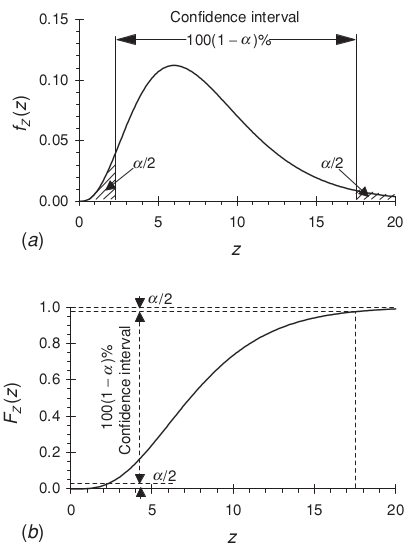
\includegraphics[width=\textwidth]{fi535.png}
\end{minipage}

\end{block}
\end{frame}


%-------
% From Kotte
\section{Hypothesis testing}
\begin{frame}{Hypothesis testing}
    \begin{itemize}
        \item A second major area of statistical inference is the \alert{testing of hypotheses}, which is closely related to the determination of \emph{confidence limits}. 
        \item What we are examining concerns the parameters or form of the probability distribution that yields the observations.
        \item This involves making a declaration or statement called a \alert{hypothesis} about a population.
        \item The discussion is focused on certain assumptions (regarding, for instance, the mean of the population) without initially making any commitment on assuming them.
        \item From a philosophical viewpoint, our conception of the actual state of nature may not be correct. However, we have a sample of data that represents the physical reality, and although our initial hypothesis may be somewhat tentative, we can revise the concept each time new information becomes available and thus come closer to the true state of nature.
        \item The approach we follow is akin to the verification of some of the scientific hypotheses of scientists and engineers. For instance, it is usually feasible to ascertain whether a procedure for treating wastewater makes a change in the quality of the effluent, as measured, for example, by the biochemical oxygen demand. As another example, there may be reason to believe that the distribution of high flows in a river has changed on account of climatic effects or because the flow regime has been altered.
    \end{itemize}
\end{frame}

\begin{frame}{Hypothesis testing}
    \begin{itemize}
        \item A random sample is taken from the population and \alert{statistical hypotheses}, called \alert{null} and \alert{alternative}, are declared. Then a statistical test is made.
        \item If the observations do not support the model or theory postulated, the \emph{null hypothesis} is \alert{rejected} in favor of the alternative one, which may be considered to be true. However, if the observations are in agreement, then the null hypothesis is \alert{not rejected}.
        \item This does not necessarily mean that it is accepted. It suggests that there is insufficient evidence against the \emph{null hypothesis} in favor of the alternative one.
        \item Associated with the decision is a \alert{level of significance}, $\alpha$. This is complementary to the probability introduced  for setting confidence limits.
        \item For instance, an engineer may question whether there has been a significant change, for instance, in a mean rate of traffic flow on a highway or an average strength of a material. On the contrary, such a variation may sometimes be due to sampling differences without any change in the mean or other aspect of the population. It is then said to be \alert{not significant}.
        \item Hypothesis testing thus concerns procedures for rejecting a statement or not rejecting it and the chances of making incorrect decisions of either kind. It also involves the use of a particular function of the sample measurements.
        \item If we assume that the observations come from a normal or other specified population, then the test is called \alert{parametric}. In contrast, \alert{nonparametric tests} are not based on such assumptions.
    \end{itemize}
\end{frame}

\begin{frame}{Hypothesis testing}

    \begin{block}{Procedure for testing}
    \end{block}
    \vspace{-5pt}
    The basic steps for hypothesis testing are listed below. Note that two different \emph{hypotheses} are compared.
    \begin{enumerate}
        \item \alert{Declare a null hypothesis, $H_0$}:  This is the hypothesis to be tested and it assume that the observed results are due to chance. For instance we may wish to verify whether the initial mean $\mu_1$ of the annual maximun flows at a river gauge station is indeed the same as a projected new mean $\mu_2$ consequent to changes in the flow regime  that may have proved sufficient for a change in the population mean. If $H_0$ is true, any observed difference in the means is merely the consequence of sampling variation from the sample population. This means that the differences are attributed to errors in random sampling. The hypothesis is expressed as: $H_0: \mu_1 - \mu_2 = 0$.
        \item \alert{Declare the alternate hypothesis, $H_1$}: This is the hypothesis that we want to test. For the previous example, this is $H_1 : \mu_1 - \mu_2 \neq 0$.
        \item \alert{Specify a test statistic}: In the previous example, the test is based on the difference between the respective observed means $\bar{X}_1$ and $\bar{X}_2$. 
        \item \alert{Determine the distribution of the test statistic}: The sampling distribution depends on the distribution to which the observations belong. Thus, we may need to make asumptions regarding the underlaying distribution. 
        \item \alert{Define a rejection/critical region for the test statistic}: For this, it is necessary to preassign a level of significance $\alpha$. 
        \item \alert{Use the observed data to verify  whether the computed value of the test statistic is within or outside the rejection region}: If this is within the rejection region we say that the difference (for the previous example) is \emph{significant at the} $100\alpha$ \% level.  
    \end{enumerate}
\end{frame}

\begin{frame}{Hypothesis testing}

    \begin{block}{Procedure for testing}
    \end{block}
    \vspace{-5pt}
    Some aspects related to the procedure for testing for the given example:
    \begin{itemize}
        \item As the \emph{rejection region} covers \emph{both tails} of the \emph{sampling distribution}, this procedure is called a \alert{two-tailed test}.
        \item If the test were something like wheather $\mu_1 > \mu_2$ \alert{one-tailed test} is requiere as the critical \emph{rejection region} cover only one tail. 
        \item If \emph{test statistic} and the \emph{rejection region} are defined as $T$ and $R$, respectively, the probability of rejecting $H_0$ is $Pr\left[T \in R | H_0\right] = \alpha$
        \item Note that the probability $\alpha$ provides the link between the \emph{confidence intervals} and \emph{hypothesis testing}.
        \item We can say that \emph{rejection} is the same as stating that the \emph{test statistics} is statistically significant.
        \item Errors:
            \begin{enumerate}
                \item \alert{Type I error}: This occurs if a hypothesis is rejected when it should be accepted, regarging that $H_0$ is true. The probability of this is $Pr \left[ \text{Type I error} \right] = Pr\left[T \in R | H_0\right] = \alpha$.
                \item \alert{Type II error}: This occurs if we fail to reject $H_0$ when it is not true. The probability of this is $Pr \left[ \text{Type II error} \right] = Pr\left[T \in A | H_1\right] = \beta$. Note that $A$ is the accptance region of the test statistic, so that $A$ and $R$ comprise the parameter space $\Omega$ for $T$. 
            \end{enumerate}
 In either of the cases, we are wrong in our judgement. Accordingly, we are right in two cases:
           \begin{enumerate}
               \item Contrary to \emph{Type I error}, if we correctly fail  to reject $H_0$, the probability is $1- Pr \left[ \text{Type I error} \right] = Pr\left[T \in A | H_0\right] = 1-\alpha$. Note that this is the same probability associated with the \emph{confidence interval}. 
               \item Contrary to \emph{Type II error}, the probability of correctly rejecting $H_0$ when it is not true is $1- Pr \left[ \text{Type II error} \right] = Pr\left[T \in R | H_1\right] = 1-\beta$
            \end{enumerate}
    \end{itemize}
\end{frame}

\begin{frame}{Hypothesis testing}

    \begin{exampleblock}{Change in  the mean annual maximum flow}
Annual maximum flows in the Pond Creek catchment area in the eastern United States are listed below in cubic meters per second for two periods of 12 years from 1945 to 1968. It is thought that changes in the flow regime during the middle of this period have modified the distribution of flows resulting in higher maximum flows. This is equivalent to stating that the mean flow has increased from the first period to the second period.
\setlength{\tabcolsep}{1pt} % global adjustment
  \begin{tabular}{rcccccccccccc}
      First period (1945-1956): & 2000 & 1740 & 1460 & 2060 & 1530 & 1590 & 1690 & 1420 & 1330 & 607 & 1380 & 1660 \\
Second period (1957-1968): & 2290 & 2590 & 3260 & 2490 & 3080 & 2520 & 3360 & 8020 & 4310 & 4380 & 3220 & 4320
  \end{tabular}
    \alert{Case 1: Known standard deviation and prior mean}\\
    \emph{Null hypothesis},$H_0 : \mu_1 = 1539$. This means that the new mean (second period mean) is equal to the past mean (1539 m$^3$/s).\\
    \emph{Alternate hypothesis},$H_1 : \mu_1 > 1539$. This means that the new mean (second period mean) is greater than the past mean (1539 m$^3$/s).\\
    \emph{Level of significance}, $\alpha = 0.01$ \\
    During the first period, the mean and the standard deviation are 1539 m$^3$/s and 372 m$^3$/s, respectively. We assume that these values  represent the population mean $\mu$ and standard deviation $\sigma$ prior to 1957. We also assume that standard deviation does not change. As we want to know whether the mean has increased, we use a \emph{one-tailed test}. 
    Let $\bar{X}$ the estimate to the mean after 1956 based on a sample size $n=12$. Assuming that the annual maximum flows follow a \emph{normal distribution}, the \emph{standard normal score} is $Z = \frac{\bar{X} - \mu}{\sigma/\sqrt{n}}$. This becomes our \emph{test statistic}. \\
    
    \end{exampleblock}

\end{frame}

\begin{frame}{Hypothesis testing}

    \begin{exampleblock}{Change in  the mean annual maximum flow}
   So for $\alpha = 0.01$ our decision rule is:
    \begin{enumerate}
        \item \emph{Reject} $H_0$ if the $z > 2.326$. 2.326 is taken from the \emph{normal distribution cdf} table for $F(x) = 1-\alpha = 0.99$.
        \item Otherwise \emph{do not reject} $H_0$. 
    \end{enumerate}
    Substituting in $Z$ for $\bar{X} = 3653$ m$^3$/s, the $z$ score is 19.7, which is much greater that 2.326. \emph{Decision: $H_0$ is rejected}.

    \alert{Case 2: Known prior mean and unknown but constant standard deviation}\\
    In practice we do not know the standard deviation. This means that the test will be based on the sample value and thus it is thus appropriate to apply the \emph{t distribution}. As before, we assume that the standard deviation is constant and that the annual maximum flows are \emph{normally distribute}. The \emph{test statistic} is $T = \frac{\bar{X}-\mu}{\sigma/\sqrt{n}}$.\\
   So for $\alpha = 0.01$ our decision rule is:
    \begin{enumerate}
        \item \emph{Reject} $H_0$ if the $t > t_{11,0.01}$, where $t_{11,0.01} =  2.718$. This value is taken from the \emph{t distribution cdf} table for $F(t) = 1-\alpha = 0.99$ and $\nu=n-1=11$. 
        \item Otherwise \emph{do not reject} $H_0$. 
    \end{enumerate}
    Substituting in $T$, the sample $t$ score is 19.7, which is much greater that 2.718. \emph{Decision: $H_0$ is rejected too}.
    \end{exampleblock}

\end{frame}

\begin{frame}{Hypothesis testing}
    Three cases of interest:
    \begin{itemize}
        \item \alert{TESTING THE DIFFERENCE BETWEEN TWO MEANS USING KNOWN VARIANCES}\\
            If $\bar{X}_1$ and $\bar{X}_2$, say, are two estimated means of $\mu_1$ and $\mu_2$ obtained from two small samples of sizes $n_1$ and $n_2$, respectively, and if the two populations are normal with known variances $\sigma_1^2$ and $\sigma_2^2$, then the random variable:
            \[
                Z = \frac{(\bar{X}_1 - \bar{X}_2) - (\mu_1 - \mu_2)}{\sigma_{\bar{X}_1 - \bar{X}_2}}
            \]
            follow a $N \sim (0,1)$. The standard error of the difference between two statistics is defined as $\sigma_{\bar{X}_1 - \bar{X}_2} = \sqrt{\frac{\sigma_1^2}{n_1} + \frac{\sigma_2^2}{n_2}}$.


        \item \alert{TESTING THE DIFFERENCE BETWEEN TWO MEANS WHEN THE VARIANCES ARE UNKNOWN BUT EQUAL}\\
            Let the sample variances be $\hat{S}_1^2$ and $\hat{S}_2^2$. Because both are estimates of the constant variance $\sigma^2$, a pooled estimate can be formed by
            \[
                \hat{S}_p^2 = \frac{(n_1 -1)\hat{S}_1^2 + (n_2 -1) \hat{S}_2^2}{n_1 + n_2 -1}
            \]
            Then, the random variable:
            \[
                T = \frac{(\bar{X}_1 - \bar{X}_2) - (\mu_1 - \mu_2)}{\hat{S}_p \sqrt{(1/n_1) + (1/n_2)}} = \frac{(\bar{X}_1 - \bar{X}_2) - (\mu_1 - \mu_2)}{\sqrt{(n_1-1)\hat{S}_1^2 + (n_2-1)\hat{S}_1^2}} \sqrt{\frac{(n_1 + n_2 -2)n_1 n_2}{n_1 + n_2}} 
            \]
            has the \emph{t distribution} with $n_1 + n_2 -2$ degrees of freedom.

    \end{itemize}

\end{frame}

\begin{frame}{Hypothesis testing}
   \begin{itemize}
        \item \alert{TESTING THE DIFFERENCE BETWEEN TWO MEANS WHEN THE VARIANCES ARE UNKNOWN AND UNEQUAL}\\
There are many instances when it is not correct to assume that the variances corresponding to the means tested are equal. However when the variances are unequal, the statistic does not have a t distribution. In the case of observations taken from normal populations with unknown and unequal variances, the statistic
\[
    T' = \frac{(\bar{X}_1 - \bar{X}_2) - (\mu_1 - \mu_2)}{\sqrt{\hat{S}_1^2 /n_1 - \hat{S}_2^2 /n_2}} 
\]
has an approximate t distribution with
\[
    \nu = \frac{\left[ \hat{S}_1^2 /n_1 - \hat{S}_2^2 /n_2 \right]^2}{ (\hat{S}_1^2 /n_1)^2 / (n_1-1) + (\hat{S}_2^2 /n_2)^2 /(n_2 -1) }
\]
degrees of freedom.
    \end{itemize}

    \begin{exampleblock}{Change in  the mean annual maximum flow with unkwnon and unequal variance}

    \emph{Null hypothesis},$H_0 : \mu_1 = \mu_2$. This means that the new mean (second period mean) is equal to the past mean (1539 m$^3$/s).\\
    \emph{Alternate hypothesis},$H_1 : \mu_1 > \mu_2$. This means that the new mean (second period mean) is greater than the past mean (1539 m$^3$/s).\\
    \emph{Level of significance}, $\alpha = 0.01$ \\
    Using the data from the previous example, for a one-tailed test
\[
    \bar{x}_1 = 1539 \quad \hat{s}_1 = 372 \quad \bar{x}_2 = 3653 \quad \hat{s}_2 = 1563 \quad n_1 = n_2 = 12
\]

    \end{exampleblock}
\end{frame}

\begin{frame}{Hypothesis testing}
    \begin{exampleblock}{Change in  the mean annual maximum flow with unkwnon and unequal variance}

        \[
            \nu = \frac{\left[(372^2 / 12) + (1563^2 / 12) \right]^2}{ \left[(372^2 / 12)^2 /11\right] +  \left[(1563^2 / 12)^2 /11\right]} \approx  12
        \]

        \[
            T' = \frac{(3653-1539)}{\sqrt{(372^2 / 12) + (1563^2 / 12)}} = 4.56
        \]
        From the \emph{t distribution} test table, $t_{12, 0.01} = 2.681$. \emph{Decision: $H_0$ is rejected too}.

    \end{exampleblock}
\end{frame}

\begin{frame}{Hypothesis testing}
    \begin{block}{Probabilities of Type I and Type II Errors and the Power Function}
    \end{block}
    As we know, the Type I error probability is $\alpha$, while the the Type II error probability depends on $\alpha$, the sample size, the true value of the parameter tested. Consider the two-tailed test used for testing the mean of a $N(\mu, \sigma^2)$ population: \emph{Null hypothesis $H_0: \mu = \mu_0$} and \emph{Alternative hypothesis $H_1: \mu \neq \mu_0$}. Suppose that is correct to reject $H_0$ because the true value of $\mu$ is $\mu_0 +c $, where $c$ is a constant. Accordingly, it is also correct to accept the alternative hypothesis with standardized test statistic $Z \sim (c\sqrt{n}, 1)$, where $n$ is the size of the test sample. Note that the mean has been displaced by $c/(\sigma /\sqrt{n})$

    \centering
    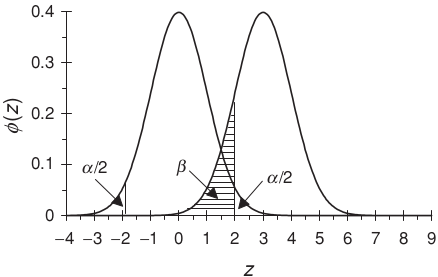
\includegraphics[width=0.7\textwidth]{fi541.png}
\end{frame}

\begin{frame}{Hypothesis testing}
    \begin{block}{Probabilities of Type I and Type II Errors and the Power Function}
    \end{block}
    The \emph{Type II error} is made when $H_1$ is true, only if $-z_{\alpha/2} \leq Z \leq z_{\alpha/2}$ where $-z_{\alpha/2}$ and $z_{\alpha/2}$ are the values which a standard normal deviate exceeds with probabilities of $(1 - \alpha/2)$ and $\alpha/2$, respectively. The probability  $\beta$ of a \emph{Type II error} is determined after adjusting the specified limits by the mean of the Z variate. Accordingly it is given by:
    \[
        \beta = \Phi \left( z_{\alpha/2} - \frac{c\sqrt{n}}{\sigma} \right) - \Phi\left( -z_{\alpha/2} - \frac{c\sqrt{n}}{\sigma} \right) 
    \]

    where $\Phi(.)$ is the \emph{cdf} of the \emph{standard normal distribution}.

\begin{minipage}[t]{0.58\textwidth}
   \vspace{0pt} % prevent extra spacing at top

   Thus we see that the probability $\beta$ of a \emph{Type II error} is dependent on $\alpha$, $n$, and $c/\sigma$ .Curves representing $\beta$ are called \alert{characteristic curves}. These are shown in the figure for a two-tailed normal test with level of significance $\alpha = 0.05$, sample sizes $n$ from 1 to 100 and $c/\sigma =$ 0.25, 0.50, 0.75, and 1.0. From these curves we see that, for the same sample size $n$, $\beta$ increases as $c/\sigma$ decreases. That is, small differences in the mean are more difficult to detect and lead to a higher probability of incorrect acceptance. Also, as expected, there is an increase in $\beta$ as the sample size $n$ decreases
\end{minipage}
\begin{minipage}[t]{0.38\textwidth}
   \vspace{0pt} % prevent extra spacing at top

    \centering
    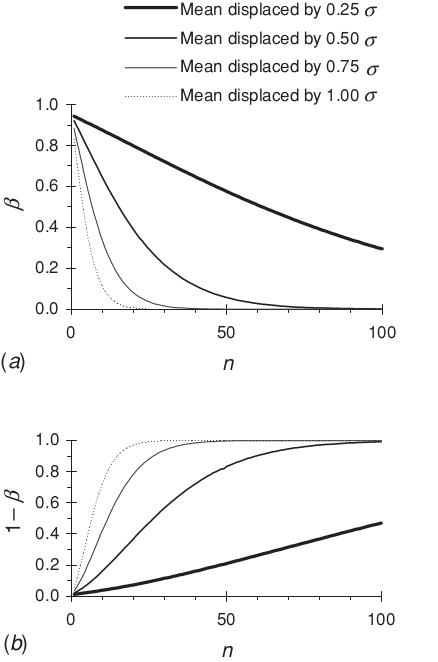
\includegraphics[width=0.8\textwidth]{fi542.png}
\end{minipage}

\end{frame}

\begin{frame}{Hypothesis testing}
    \begin{block}{Probabilities of Type I and Type II Errors and the Power Function}
    \end{block}
    The complement of $\beta$ is the \alert{power function}. As already stated it is the \emph{probability of rejecting the null hypothesis when it is not true } (which is of course the right thing to do) in favor of the alternative hypothesis. It is equivalent to $\text{Power } = 1 - \beta$. Power curves are shown in the previous figure for a two-tailed normal test with level of significance $\alpha = 0.01$, sample sizes $n$ from 1 to 100 and $c/\sigma = $ 0.25, 0.50, 0.75, and 1.0. Clearly, the power increases with $c/\sigma$ and sample size $n$.
\end{frame}

\begin{frame}{Hypothesis testing}
    \begin{block}{Neyman-Pearson lemma}
    \end{block}
Here we are concerned with the behavior of observable random variables. For example, if a random sample is taken from a distribution with specific parameters, then a simple hypothesis is one that uniquely defines the distribution from which the sample is taken against an alternative hypothesis.

    Let $R$ be a critical (rejection) region of size $\alpha$, when testing the null hypothesis $H_0 : \theta = \theta_0$ against the alternative hypothesis $H_1 : \theta = \theta_1$. We define a constant $k_{\alpha}$ such that in the region $R$, $(L_0 /L_1 )\leq k_{\alpha}$ , and in the acceptance region $A$, $L_0/ L_1 > k_{\alpha}$, where $L_0 = \prod_{i=1}^n f (x_i | \theta_0 )$ and $L_1 = \prod_{i=1}^n f (x_i | \theta_1 )$ . Then $R$ is the \emph{best critical region (bcr)} of size $\alpha$. Such a test involving a \emph{bcr} is called a \emph{most powerful (mp) test}.

    \begin{exampleblock}{A simple likelihood test on a normal population with unit variance}
        Let $X_1 , X_2 , \cdots, X_n$ be a random sample from an $N (\mu, 1)$ population. Suppose our objective is to test the $H_0 : \mu = \mu_0$ against the alternative hypothesis $H_1 : \mu = \mu_1 > \mu_0$ . The ratio of the likelihoods can be used to find the \emph{bcr} of size $\alpha$, and the ratio is
        \[
            \frac{L_0}{L_1} = \frac{(1/\sqrt{2 \pi})^n e^{\left[-1/2 \sum_{i=1}^n ( X_i - \mu_0 )^2 \right]}}{(1/\sqrt{2 \pi})^n e^{\left[-1/2 \sum_{i=1}^n ( X_i - \mu_1 )^2 \right] }} = e^{\left[ \left(\sum_{i=1}^n X_i \right) (\mu_0 - \mu_1) + \frac{n}{2} \left( \mu_1^2 - \mu_0^2 \right) \right]}
        \]
    \end{exampleblock}
\end{frame}

\begin{frame}{Hypothesis testing}
    \begin{block}{Neyman-Pearson lemma}
    \end{block}
    \begin{exampleblock}{A simple likelihood test on a normal population with unit variance}
        We define a constant $k_{\alpha}$ , which depends on $\alpha$, as a limiting value of the likelihood ratio, and a critical region $R$ of size $\alpha$ within which
        \[
            e^{\left[ \left(\sum_{i=1}^n X_i \right) (\mu_0 - \mu_1) + \frac{n}{2} \left( \mu_1^2 - \mu_0^2 \right) \right]} \leq k_{\alpha}
        \]
        Outside $R$,

        \[
            e^{\left[ \left(\sum_{i=1}^n X_i \right) (\mu_0 - \mu_1) + \frac{n}{2} \left( \mu_1^2 - \mu_0^2 \right) \right]} \geq k_{\alpha}
        \]
        Taking logarithms and simplifying, we find for $H_1 : \mu = \mu_1 > \mu_0$ , the \emph{bcr} is defined for
        \[
            \bar{X} \geq \frac{1}{2} (\mu_0 + \mu_1) - \frac{\ln k_{\alpha}}{n(\mu_1 - \mu_0)} = c_{\alpha}
        \]


        If the alternate hypothesis is $H_1 : \mu = \mu_1 < \mu_0$ , the \emph{bcr} is defined for

        \[
            \bar{X} \leq \frac{1}{2} (\mu_0 + \mu_1) + \frac{\ln k_{\alpha}}{n(\mu_0 - \mu_1)} 
        \]
    \end{exampleblock}
\end{frame}

\begin{frame}{Hypothesis testing}
    \begin{block}{Tests of hypotheses involving the variance}
    \end{block}
    In equation 

\[
    Pr \left[ \chi^2_{n-1, 1- \alpha/2} \leq \frac{(n-1)\hat{S}^2}{\sigma^2} \leq  \chi^2_{n-1, \alpha/2} \right] = 1-\alpha
\]
    we noted that a quantity such as $\sum_{i=1}^n (X_i - \bar{X} )^2 /\sigma^2$ has a \emph{chi-squared distribution} with $(n - 1)$ degrees of freedom. However, if the true mean $\mu$ is known, this replaces $\bar{X}$ in the preceding sum of squares and the degrees of freedom are $n$. Thus with the knowledge of the sampling distribution, a hypothesis test can be made on the variance.

    \begin{exampleblock}{A significance test on the change in variance}
        From a long series of annual river flows, the variance is found to be 49 units. This can be treated as the population variance. However, a new sample of 25 years gives a value $\hat{s}^2 =$ 81 units. So $H_0 : \sigma^2 = 49$, $H_1 : \sigma^2 = 49$ and $\alpha = 0.05$. 
        The quantity $n \hat{s}^2/\sigma^2$ has a \emph{chi-squared distribution} with $n$ degrees of freedom. From the \emph{chi-squared distribution} for $\chi_{25,0.05}^2 = 37.7$ and $n \hat{s}^2 / \sigma^2 = 25 x 81/49 = 41.3$. \emph{Decision: $H_0$ is rejected}.  
    \end{exampleblock}
\end{frame}

%-------
% From Kotte
\section{Nonparametric methods}
\begin{frame}{Nonparametric methods}
    Some generalities:
    \begin{itemize}
        \item The \emph{normal distribution} plays a central role in the theory of statistics and probability and its use is supported by the \emph{Central Limit Theorem}.
        \item However, there are many instances when one is uncertain of the true form of the \emph{probability distribution} of the variable involved and the available sample is small, say, less than 30.
        \item It is therefore desirable to have methods that can be applied regardless of distribution. Such procedures are called \alert{distribution-free methods}.
        \item The term \alert{nonparametric methods} is generally used to describe the wide-ranging procedures. In these methods we are not concerned with the parameters of populations.
        \item In contrast, \alert{parametric methods} pertain to those techniques where the distribution is known but the values of the parameters are not specified.
        \item Furthermore, \alert{nonparametric methods} do not require much computational effort and are thus easier to apply. Also, small samples can be used.
        \item Although the methods are less powerful in detecting \emph{Type I and Type II errors}, the \emph{loss of power} is sometimes minimal and is outweighed because the assumptions are less restrictive.
    \end{itemize}
\end{frame}

\begin{frame}{Nonparametric methods}

    \begin{block}{Sign test applied to the median}
    \end{block}
    The \alert{one sample sign test} is applicable when we sample any continuous distribution that has a \emph{median, $M$}. We test the hypothesis that the \emph{median} is equal to a specific value $M_0$. Let $n$ be the number of nonzero differences between the sample values and the assumed median, which is true under the null hypothesis, and let $k$ be the number of positive differences. Then by the \emph{normal approximation} to the \emph{binomial}, the following variate has a \emph{standard normal distribution} under the null hypothesis:
    \begin{align*}
        z &= \frac{(k + 1/2)-n/2}{1/2 \sqrt{n}}, \text{ if } k < \frac{n}{2} \\
        z &= \frac{(k - 1/2)-n/2}{1/2 \sqrt{n}}, \text{ if } k > \frac{n}{2} \\
    \end{align*}
    The $z_{\alpha}$ value from the \emph{normal cdf} table is compared with the $z$ score calculated from one of the preceding equations to decide whether the \emph{null hypothesis} should be rejected at a level of significance $\alpha$. Note that the null hypothesis to be testes if $H_0 : M = M_0$, and the alternative hypothesis is one of the following: $H_1 : M < M_0$ or $H_1 : M > M_0$. 
    %The \alert{nonparametric sign test} is an alternative to the tests on the \emph{mean} using the \emph{normal or the t distribution} as sampling distributions.
    \end{frame}

\begin{frame}{Nonparametric methods}

    \begin{block}{Wilcoxon signed-rank test for association of paired observations}
    \end{block}
    In the \emph{sign test} we make use of only the signs of the differences between the observations and the \emph{median}. The \alert{Wilcoxon signed-rank test} utilizes the magnitudes of the differences and is thus intuitively a more powerful test compared with the much simpler \emph{sign test}. Both procedures can be used in testing differences in \emph{means}.
    \begin{enumerate}
        \item We note the magnitudes and the signs of the paired differences from two samples of observations.
        \item The absolute values of the differences are ranked. Here, the smallest difference is assigned rank 1 and the largest difference gets the highest rank, which is equal to the number of pairs $n$ with nonzero differences.
        \item If the absolute values of two or more of such differences are equal, we give each a rank equal to the mean of the ranks they would otherwise receive.
        \item The ranks attributed to positive and negative differences are then summed in separate columns. These sums are denoted $T^+$ and $T^-$ , respectively.
    \item While $H_0 : \mu_1 = \mu_2$, the$H_1 : \mu_1 < \mu_2$ or $H_1 : \mu_1 > \mu_2$. 
    \end{enumerate}
    Under the \emph{null hypothesis} we can use either $T^+$ or $T^-$, the sum of the ranks applied to the absolute values of the positive and negative differences, respectively, between the paire observations for the \emph{test statistic T}. For large sample sizes $n$, $T$ can be approximate by the \emph{standard normal variate} $Z =\frac{T - \mu_T}{\sigma_T} $, where $\mu_T = \frac{n(n+1)}{\sigma_T}$ and $\sigma_T^2 = \frac{n(n+1)(2n+1)}{24}$.

    The $z_{\alpha}$ value from the \emph{normal cdf} table is compared with the $z$ score calculated from   the preceding equation to decide whether the \emph{null hypothesis} should be rejected at a level of significance $\alpha$. Note the approximation is sufficiently accurate for $n \geq 15$.
    \end{frame}

\begin{frame}{Nonparametric methods}
    \begin{block}{Kruskal-Wallis test for paired observations in $k$ samples}
    \end{block}
    \begin{itemize}
        \item The test is applied to, say, $k$ independent \emph{random samples} of sizes $n_i$ , $i = 1, 2, \dots , k$, with a total of $n$ observations.
        \item It is assumed that all samples are \emph{random samples} from their individual populations and that there is independence within the samples and between them.
        \item The null hypothesis is that the samples come from the same continuous population. The alternate hypothesis is that at least one of the populations tends to produce comparatively larger values than the others.
        \item Following a procedure similar to that in the \emph{Wilcoxon signed-rank}, the pooled data are ranked from the lowest to the highest as if they belong to one sample.

    \end{itemize}
    If $R_i$ is the sum of the ranks of the data in the $ith$ sample of size $n_i$ and $n$ is the total sum of the $k$ samples, the normalized test statistic is $H = \frac{12}{n(n+1)} \sum_{i=1}^k \frac{R_i^2}{n_i} - 3(n+1)$. Under the \emph{null hypothesis} that the samples come from the same population, $H$ has an approximate \emph{chi-squared distribution} with $(k - 1)$  \emph{degrees of freedom}.
   \end{frame}

\begin{frame}{Nonparametric methods}
    \begin{block}{Tests on randomness: runs test}
    \end{block}
    \begin{itemize}
        \item In the applications of statistical methods, it is often assumed that a sample is taken at random and that the values of a sample represent variables that are themselves random.
        \item A technique based on the \emph{number of runs } shown by a series is applicable as a general test on randomness.
        \item A \alert{run} is a sequence of variables of a particular kind that is preceded and followed by a sequence of variables of a different kind or by no variables at all.
        \item For example, \emph{magnitudes greater} than the \emph{median} can be of one kind, in which case \emph{magnitudes below} the \emph{median} will constitute the other kind.
        \item As an illustration, consider the following series which represents 35 pollutant levels in a stream measured at regular intervals of time denoted by either $A$, \emph{acceptable}, or $U$ , \emph{unacceptable}:
            \[
U \, U  \, A  \ U  \ A  \ U  \ U  \ U  \ U  \ U  \ A  \ A  \ U  \ U  \ U  \ U  \ A  \ U  \ A  \ A  \ A  \ A  \ U  \ U  \ A  \ A  \ A  \ A  \ A  \ U  \ A  \ A  \ U  \ U  \ A 
\]
\item By the given definition, this comprises 16 runs where, for example, each run of one or more $U$s is preceded and followed by a run of one or more $A$s or no measurements at all.
\item In such cases, the total number of \emph{runs} relative to the \emph{sample size} provides an indicator of \emph{randomness}. Too few runs suggest a \emph{grouping}, \emph{clustering}, \emph{trend}, or \emph{periodic} behavior, whereas too many runs lead to the suspicion that there are \emph{high-frequency oscillations}. A random series should have neither too few nor too many runs.
    \end{itemize}

    \end{frame}

\begin{frame}{Nonparametric methods}
    \begin{block}{Tests on randomness: runs test}
    \end{block}
    In a sequence containing $n$ variables of one kind and $m$ variables of another kind, the sampling distribution of the total number of runs, $R$, can be closely approximated by the normal distribution with $\mu_R = 1 + \frac{2nm}{(n+m)}$ and $\text{Var}[R] = \frac{2nm(2nm - n - m)}{(n+m)^2 (n+m-1)}$. The approximation is quite close for  $m, n>9$
    \begin{exampleblock}{Runs test on annual river flows}
        Annual flows  for the period 1938-1967 are tabulated below in millimetres of equivalent runoff over the catchment area above the site.
        \vspace{5pt}

  \begin{tabular}{rrrrrrrrrr} % no | bars, no \hline
      946 & 1074 & 867 & 1058 & 838 & 837 & 1133 & 815 & 1138 & 869 \\
      910 & 868 & 927 & 1193 & 969 & 742 & 1386 & 737 & 1113 & 955 \\
      1143 & 665 & 1187 & 947 & 955 & 891 & 763 & 1288 & 1302 & 1029
  \end{tabular}

  Our objective is to ascertain whether the population is random using the \emph{runs test}.
    \emph{Null hypothesis},$H_0$ : The population is random.\\
    \emph{Alternate hypothesis},$H_1$  : The population is not random.\\
    \emph{Level of significance}, $\alpha = 0.05$\\
    The \emph{median} is 951 mm and the \emph{runs} above the \emph{median} are underlined as follows:
         \vspace{5pt}

  \begin{tabular}{rrrrrrrrrr} % no | bars, no \hline
      946 & \underline{1074} & 867 & \underline{1058} & 838 & 837 & \underline{1133} & 815 & \underline{1138} & 869 \\
      910 & 868 & 927 & \underline{1193} & \underline{969} & 742 & \underline{1386} & 737 & \underline{1113} & \underline{955} \\
      \underline{1143} & 665 & \underline{1187} & 947 & \underline{955} & 891 & 763 & \underline{1288} & \underline{1302} & \underline{1029}
  \end{tabular}

 
    \end{exampleblock}
 
    \end{frame}


\begin{frame}{Nonparametric methods}

    \begin{exampleblock}{Runs test on annual river flows}
  The number of values $n$ \emph{above the median} equal the number of values $m$ \emph{below the median}, 15. The total number of observed \emph{runs} $r = 20$. The test statistic is:
  \[
      Z = \frac{(R \pm (1/2) )- \mu_R}{\sqrt{Var[R]}}
      \]
      By using a two-tailed test with $\alpha = 0.05$, the \emph{critical region} is $Z$ (positive with $R + 1/2$) $>$ 1.96 and $Z$ (negative with $R - 1/2$) $<$ -1.96, from  the \emph{normal cdf}. Sample estimates of the \emph{mean} and the \emph{variance} of the total number of runs are:
      \[
          \mu_R = 1 + \frac{2 x 15 x 15}{30} = 16 \quad \text{and} \quad Var[R] = \frac{2 x 15 x 15(450-30)}{30^2 x 29} = 7.24
      \]
      Hence,
      \[
          z = \frac{(20 + 1/2) - 16}{\sqrt{7.24}} = 1.49
      \]
\emph{Decision: the null hypothesis that the population is random is not rejected}.
    \end{exampleblock}
    \end{frame}

\begin{frame}{Nonparametric methods}

    \begin{block}{Spearman’s rank correlation coefficient}
    \end{block}
    \alert{Spearman's rank correlation coefficient}; it is often referred to simply as the \emph{rank correlation coefficient}.That is, the data are converted to ranks.  \emph{Spearman's rank correlation coefficient} is estimated as follows for a set of paired data, $(x_i , y_i)$, $i = 1, 2, \cdots, n$, that are ranked separately so that, for each data set, the highest value has rank 1 and rank $n$ is that of the lowest value:
    \[
        r_s = 1 - \frac{6\sum_{i=1}^n d_i^2}{n(n^2 -1)}
    \]
    where $d_i$ is the difference between the ranks given to $x_i$ and $y_i$. Under the \emph{null hypothesis} of no correlation between the $X$ and $Y$ series, the distribution of $r_s$ can be closely approximated by the \emph{normal distribution} with $\mu_{r_s} = 0$ and $Var[r_s ] = 1/(n-1)$.
    \end{frame}

%-------
% From Kotte
\section{Goodness-of-fit tests}
\begin{frame}{Goodness-of-fit tests}

    \begin{block}{Generalities}
    \end{block}
        \begin{itemize}
            \item \emph{Hypothesis-testing} procedures related to the \emph{parameters} of a distribution.
            \item Another important type of hypothesis concerns the \emph{form of a probability distribution}. It may, for example, be necessary to test whether a \emph{discrete variable} has a \emph{Poisson distribution} or whether a \emph{continuous variable} is \emph{normally distributed}.
            \item For these purposes, we may compare \emph{observed} and \emph{theoretical cumulative frequencies}.
            \item To test that, there are some two main types of \alert{goodness-of-fit tests}.
        \end{itemize}

    \end{frame}

\begin{frame}{Goodness-of-fit tests}

    \begin{block}{Chi-squared goodness-of-fit test}
    \end{block}

    The \alert{chi-squared test} is a \emph{test of significance} based on the \emph{chi-squared statistic} with \emph{cdf} given by
    \[
        F(\chi^2) = \frac{1}{2} \int_0^{\chi^2} \frac{(u/2)^{(\nu/2)-1} e^{-u/2}}{\Gamma(\nu/2)} du
    \]

    Note that the \emph{statistic} is derived by the sum of squares of \emph{independent standard normal variates} $\chi^2 = Z_1^2 + Z_2^2 + \cdots + Z_n^2$. The main steps are the \emph{ranking of a sample of data}, \emph{division into a number of classes} depending on the magnitudes and the range, and the \emph{fitting of a probability distribution}. The statistic comes from the weighted sum of squared differences between the observed and theoretical frequencies.
    In the \alert{Chi-squared goodness-of-fit test},  the test statistic is
    \[
        X^2 = \sum_{i=1}^l \frac{(O_i - E_i)^2}{E_i}
    \]
    where $O_i$ and $E_i$ are the \emph{observed} and \emph{expected} (obtained from a hypothetical probability distribution) frequencies, respectively, for each class $i$ out of a total of $l$ classes into which an ordered sample of $n$ observations is placed. The \emph{sampling distribution} of $X^2$ tends, as $n$ approaches infinity, to a $\chi^2$ distribution, where $\nu = l - k - 1$ represents the \emph{degrees of freedom} and $k$ is the number of parameters estimated from the same sample as used in the test. The test is applicable to \emph{discrete and continuous variables}, with a minimum of 5 values in each class.
    \end{frame}

\begin{frame}{Goodness-of-fit tests}

    \begin{block}{Chi-squared goodness-of-fit test}
    \end{block}

    \begin{exampleblock}{Goodness-of-fit of wet runs of rainfall}
\begin{minipage}[t]{0.54\textwidth}
   \vspace{0pt} % prevent extra spacing at top
        Whereas period of consecutive rainy days is known as \emph{wet run}, a period of consecutive dry days is known as \emph{dry run}. Suppose that in a weather station, periods of wet and dry runs are extracted from daily rainfall time series between January 1958 and May 1965. It is that the \emph{geometric distribution} provides a close fit to the observed distribution of wet runs. For a formal assessment of these fits, we can use the \emph{chi-squared goodness-of-fit test}.

\end{minipage}
\begin{minipage}[t]{0.45\textwidth}
   \vspace{0pt} % prevent extra spacing at top
    \centering
    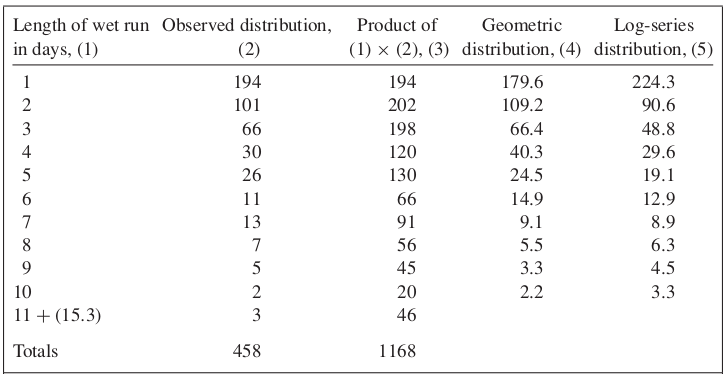
\includegraphics[width=\textwidth]{ta415.png}
\end{minipage}

     \emph{Null hypothesis}, $H_0 :$ The random variable (wet runs) has a geometric distribution with $p = 0.392$.

    \emph{Alternate hypothesis}, $H_1 :$  The random variable does not have the specified distribution.

    \emph{Level of significance}, $\alpha = 0.01$ \\

    Note that there are $l = 10$ classes and $k = 1$ (one parameter), so  gives $v = 10 - 1 - 1 = 8$. According to the values in the table, $X^2$ is 8.49. From the table of the \emph{chi-squared distribution cdf} for $\nu$ degrees of freedom, $\chi_{8,0.05}^2 = 15.5$. \emph{Decision: Because $X^2 < \chi_{8,0.05}^2$ $H_0$ is not rejected}. It is concluded that the \emph{wet runs} have a \emph{geometric distribution} as specified.
        
    \end{exampleblock}

   \end{frame}

\begin{frame}{Goodness-of-fit tests}
    \begin{block}{Kolmogorov-Smirnov goodness-of-fit test}
    \end{block}
    The \alert{Kolmogorov-Smirnov goodness-of-fit test} is a \emph{nonparametric test} that relates to the \emph{cdf} rather than the \emph{pdf} of a \emph{continuous variables} only.The \emph{test statistic}, in a \emph{two-sided test}, is the \emph{maximum absolute difference} (that is, usually the vertical distance) between the empirical and hypothetical \emph{cdfs}.

    For a continuous variate X let $x_{(1)}, x_{(2)}, \cdots, x_{(n)},$ represent the ordered (ascending order) statistics of a sample of size $n$. The empirical or sample distribution function $F_n (x)$ is a \emph{step function}. This gives the proportion of values not exceeding $x$ and is defined as:
    \begin{align*}
        F_n (x) &= 0, \quad \text{for } x < x_{(1)}\\
                &= k/n, \quad \text{for } x_{(k)} \leq x\leq x_{(k+1)}; k= 1, 2, \cdots, n-2 \\
                &= 1, \quad \text{for } x > x_{(n)}
    \end{align*}
    Let $F_0 (x)$ denote a completely specified theoretical continuous \emph{cdf}. The \emph{null hypothesis $H_0$ } is that the true \emph{cdf} of $X$ is the same as $F_0 (x)$. That is, under the null hypothesis $\lim_{n \rightarrow \infty} Pr[F_n (x) = F_0 (x)] = 1 $. 

    The  \emph{test criterion} is the maximum absolute difference between $F_n (x)$ and $F_0 (x)$, formally defined as $D_n = \underset{x}{\sup} | F_n (x) - F_0 (x) |$. For large values of $n$,  the limiting distribution of n $D_n$ , is

    \[
        \lim_{n\rightarrow \infty} \left[ \Pr [ \sqrt{n} D_n \leq z] \right]=\left( \frac{\sqrt{2\pi}}{z} \right) \sum_{k=1}^{\infty} e^{\left[-(2k-1)^2 \frac{\pi^2}{8z^2}\right]}
    \]

   \end{frame}

\begin{frame}{Goodness-of-fit tests}
    \begin{block}{Kolmogorov-Smirnov goodness-of-fit test}
    \end{block}

    Thus, one can can compute that the critical values $D_{n,\alpha}$ for large samples, say, $n > 35$, are $1.3581/\sqrt{n}$ and $1.6276/\sqrt{n}$ for $\alpha = $ 0.05 and 0.01, that is, for probabilities of 0.95 and 0.99 in equation above, respectively. Note that from simulations, note that these results hold closely for the summation of even the first five terms in the equation. For smaller sample sizes, critical values $D_{n,\alpha}$ are given in a table with values of $D_{n,\alpha}$ for the \emph{Kolmogorov-Smirnov goodness-of-fit test}.
        
   \end{frame}

\begin{frame}{Goodness-of-fit tests}
    \begin{block}{Anderson-Darling goodness-of-fit test}
    \end{block}
    The \alert{Anderson-Darling test} is devised to give \emph{heavier weighting to the tails} of a distribution where unexpectedly high or low values, called outliers are sometimes located. This is made possible if one divides the difference between the \emph{empirical cdf} $F_n (x)$ and \emph{theoretical cdf} $F_0 (x)$ to be tested by $\sqrt{F_0 (x) [1- F_0 (x)]}$. After squaring, the test statistic becomes 
    \[
        A^2 = \int_{\infty}^{\infty} \left[ F_n (x) - F_0 (x) \right]^2 \frac{1}{F_0 (x) [ 1- F_0 (x)]} f_0 (x) dx
    \]
    where $f_0 (x)$ is the \emph{hypothetical pdf}. This equation is equivalent to
    \[
        A^2 = -n - \sum_{i=1}^n \frac{(2i-1) \left[ \ln F_0(x_{(i)})+\ln(1-F_0 (x_{(n-i+1)})) \right]}{n}
    \]
    where $x_{(1)}, x_{(2)}, \cdots, x_{(n)} $ are the observations ordered in ascending order. Because the \emph{cdfs} are in the range 0-1, their logarithms are negative and hence the summation on the righthand side of the equation is negative. The absolute value of the summation is also greater than $n$, thus resulting in a positive value of $A^2$.

    For large values of the test statistic $A^2$, the \emph{ null hypothesis} that $F_n (x)$ and $F_0 (x)$ have the same distribution is rejected. From tabulated values, for large samples the values of the statistic are $A_{0.05}^2 = 2.492$ and $A_{0.01}^2 = 3.857$, for $\alpha = $ 0.05 and 0.01, respectively. These critical values of test statistic are sufficiently accurate for $n>10$.  

        
   \end{frame}

\begin{frame}{Goodness-of-fit tests}
    The following are a summary of other tests to verify the fit of a \emph{normal distribution} to an observed distribution. 
    \begin{block}{Sample skewness $g_1$ and kurtosis $g_2$}
        For the \emph{null hypothesis} $E(G_1) = 0$ and $E(G_2) = 3$. Also, the \emph{asymptotic variance} of the \emph{skewness} is $Var(G_1) = \frac{6n(n-1)}{(n-2)(n+1)(n+3)}$, which for large samples tends to $Var(G_1) =6/n$. Under the null hypothesis, the distribution of the \emph{sample skewness} $G_1$ is normal whereas that of the \emph{sample kurtosis} $G_2$ is nonnormal.

    \end{block}

    \begin{block}{Shapiro and Wilk's W-statistic}
        This is the ratio of the sum of the squares of a specified linear combination of all the ordered sample values to the sum of the squared deviations of each of the values from the sample mean $\bar{x}_n$. It is given by
        \[
        W = \frac{\sum_{i=1}^{[m]} a_{n, n+1-i} \left[ x_{(n+1-i)} - x_{(i)} \right]^2}{\sum_{i=1}^n [x_i - \bar{x}_n ]^2}  
        \]
The highest integer less than $n/2$ becomes the upper limit of summation $[m]$ in the numerator. Note that the weights $a_{n, n+1-i}$ are tabulated by many authors. 
    \end{block}
   \end{frame}

%-------
% From Diaz-Gran
\section{Detection of outliers}
\begin{frame}{Detection of outliers}

    \begin{block}{Generalities}
    \end{block}
        \begin{itemize}
            \item \emph{Outliers} are sample data that deviate significantly from the rest. These are \emph{unexpected hight or low values} in comparison to the other data, and these  are not apparently representative of the sample and thus could not come from the same distribution.  
            \item The elimination of outliers could affect the  \emph{statistical parameters} initially estimated with the original sample, even more, when the sample is small. 
            \item A first step in detecting  outliers in hydrological data is by plotting the data \emph{histogram}, \emph{Q-Q plot} and \emph{box plots}. A second step is to compute some \emph{statistics} and apply \emph{hypothesis tests}. 
            \item Two procedures are recommended to deal with \emph{outliers}:
                \begin{enumerate}
                    \item Known physical or procedural explanation of the occurrence of the outlier
                        \begin{itemize}
                            \item Reject the sample point 
                            \item Correct the sample point based on physical or procedural knowledge
                            \item Reject the sample point and replace it with a new observation
                        \end{itemize}
                    \item Unknown physical or procedural explanation of the occurrence of the outlier
                        \begin{itemize}
                            \item Reject the sample point based on statistical analysis
                            \item Correct the sample point using statistical knowledge 
                            \item Reject the data and replace it with a new observation
                        \end{itemize}
                \end{enumerate}

            \item Statistical tests can be used to assess the outlier when there is no physical or procedural reasons that cause it. 
            \item One strategy to know if a sample point is an outlier is to see if after including it, the sample point affect the analysis of interest.
        \end{itemize}
   \end{frame}

\begin{frame}{Detection of outliers}
    \vspace{-5pt}
    \begin{block}{Statistical test}
    \end{block}
    \vspace{-5pt}
    To detect outliers, we suppose that the sample data comes from a certain \emph{probability distribution}. The following tests suppose that the sample comes from  a \emph{normal distribution}.

    \begin{itemize}
        \item \alert{Z-score test}\\
            The test establishes that the sample point $Y_i$ is a potential \emph{outlier} if the absolute value of $Z_i = \frac{Y_i - \bar{Y}}{s_Y}$ is greater than 3. The test establishes how far, in term of $s_Y$, is $Y_i$ according to a \emph{normal distribution}. The maximum $Z_i$ value is $\frac{n-1}{\sqrt{n}}$, which means that the test can be applied to $n\geq 11$, otherwise $Z_{i_{max}} < 3$. The \emph{Z-score} statistic is
    \vspace{-7pt}
            \[
                M_i = \frac{0.6745 (Y_i - \tilde{Y})}{DMA}
            \]
            where $\tilde{Y}$ is the median of the data sample, and $DMA$ is the median of the absolute differences between each sample point and $\tilde{Y}$. A sample point is thus considered an \emph{outlier} if $|M_i| > 3.5$.
        \item \alert{Grubbs test}\\
            This test detects only one outlier in a data sample that follow approximately a \emph{normal distribution}. The \emph{null hypothesis $H_0$}: there is no outliers in the sample, and the \emph{alternate hypothesis $H_1$}: there is one outlier in the sample. The statistic $G = \frac{\bar{Y}-Y_{min}}{s_Y}$ or $G = \frac{Y_{max}-\bar{Y}}{s_Y}$ is calculated. The  expression of $G$ is implemented whether one want to verify either $Y_{min}$ or $Y_{max}$ of the sample. For a level of significance $\alpha$, $H_0$ is rejected if 
    \vspace{-9pt}
            \[
                G > \frac{n-2}{\sqrt{n}} \left[ \frac{t_{n-2, 0.5\alpha/n}^2 }{n-2 + t_{n-2, 0.5\alpha/n}^2}\right]
                \]

    \vspace{-3pt}
                where $n$ is the data sample size and $t_{n-2, 0.5\alpha/n}^2 $ is a critical value of the \emph{t-student distribution}.

       \end{itemize}
   \end{frame}

\begin{frame}{Detection of outliers}
    \begin{block}{Statistical test}
    \end{block}
    \vspace{-5pt}

    \begin{itemize}
        \item \alert{Tietjen and Moore test}\\
            This test serves to detect multiple outliers in a data sample that follows a \emph{normal distribution}. For this test, the \emph{null hypothesis $H_0$}: there are not outliers in the sample,  and the \emph{alternate hypothesis $H_1$}: there are $k$ outliers in the sample. The sample points are ordered from the minimum to the maximum and the following statistic is computed
            \[
                L_k = \frac{\sum_{i=1}^{n-k} (Y_i - \bar{y}_k )^2}{\sum_{i=1}^{n}  (Y_i - \bar{Y})^2} \quad \text{or} \quad L_k = \frac{\sum_{i=k+1}^{n} (Y_i - \bar{y}_k )^2}{\sum_{i=1}^{n}  (Y_i - \bar{Y})^2}
            \]
            where the equations of $L_k$ serve to verify high or low values, respectively, $\bar{y}_k$ is the average of the sample $k$ with the highest or lowest values. In either case, $H_0$ is rejected if $L_k < L_{c,\alpha}$ where $L_{c, \alpha}$ are get from a table with critical values of the \emph{Tietjen and Moore test} as a function of $\alpha$, $n$ and $k$. 

       \end{itemize}
   \end{frame}




\end{document}

%-------
% From Kotte
%\section{Analysis of variance}
%\begin{frame}{ Analysis of variance}
%
%    \begin{block}{Generalities}
%
%        \begin{itemize}
%            \item The \alert{analysis of the variance} or \alert{ANOVA} is concerned only with the variation in the means through the analysis of sums of squares. 
%            \item The methods discussed here vary from a \emph{single-factor ANOVA} to the design and analysis of results of experiments involving two or more factors with interactions between them.
%
%           \end{itemize}
%    \end{block}
%
%
%   \end{frame}


